% !TEX root = ../thesis.tex

% Tutkimustuloksien merkitystä on aina syytä arvioida ja tarkastella
% kriittisesti. Tässä osassa on syytä myäs arvioida tutkimustulosten luotettavuutta.

% At this point, you will have some insightful thoughts on your implementation
% and you may have ideas on what could be done in the future. This chapter
% is a good place to discuss your thesis as a whole and to show your professor
% that you have really understood some non-trivial aspects of the methods you
% used. . .

\documentclass[thesis.tex]{subfiles}

\begin{document}

\chapter{Discussion}
\label{chapter:discussion}

This chapter begins with a discussion of the design decisions taken during the implementation of the application, and continues by presenting the findings made from the raw result data and Chapter \ref{chapter:results}. Last, challenges faced during the project and an outline for future research work are presented, and the research questions establised in Chapter \ref{chapter:research-questions} are reviewed. Motivation behind some of the design choices referred to in the earlier chapters are not reiterated here, and the interested reader is instead advised to refer to Chapter \ref{chapter:design-implementation} and the related appendices \ref{appendix:camera-module} and \ref{appendix:capture-presets}.

\section{Design Choices}

One of the early challenges in the project was the capture of the photoexcitation. A prototype of the camera module had already been developed prior the project for demonstration purposes. It provided good isolation from ambient light and even a built-in slot for different diffraction gratings and slits. However, the prototype did not have an integrated light source, and therefore, taggants had to be excited manually by toggling a UV flashlight (Nightsearcher UV 365). For product authentication purposes a more granular, programmatic control over the light source was required. Moreover, the added benefit of using a diffraction grating and a slit to achieve higher color resolution would have been cancelled out by the loss of spatial information (taggant positioning) and its negative impact on the already low Signal-to-noise ratio (SNR). Also, as the 3D printed mold used for attaching a smartphone to the camera module prototype was designed only for Lumia 920, the integration of the Samsung S4 and Lumia 1020 would have increased the initial workload significantly. Thus, an alternative, simple and more customizable cardboard prototype was implemented, as presented in Chapter \ref{chapter:camera-module}. Figure \ref{figure:origina-camera-module} provides a wireframe of the original camera module design together with a sample image taken with a Lumia 920.

\begin{figure}[h!]
  \centering 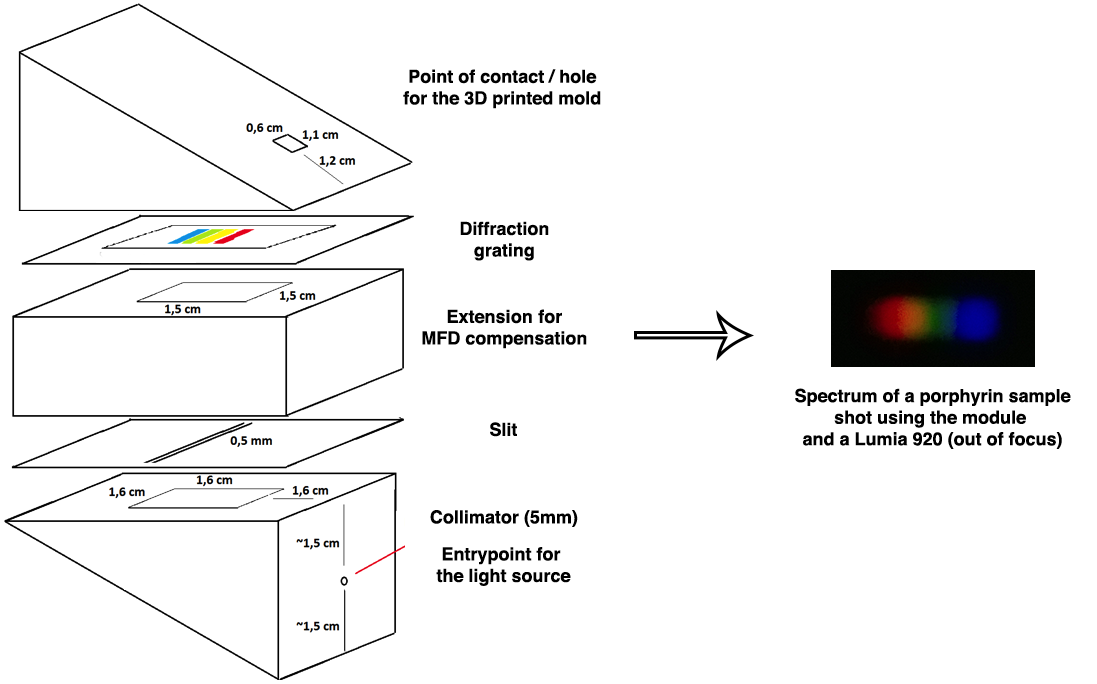
\includegraphics[page=1,width=\textwidth]{images/findings/original_camera_module}
  \caption{The design wireframe of the original camera module that included a diffraction grating and a slit. The 3D printed mold used for attaching a smartphone to the module was, however, only designed to fit a Lumia 920.}
  \label{figure:origina-camera-module}
\end{figure}

An external light source was required since the smartphone torch light in both the Samsung S4 and Lumia 1020 did not emit the right kind of light (wavelength) to be able to excite the taggants. An external light source also helped to normalize the differences between various kinds of wavelengths smartphone torch lights emit. The programmatic control of the light source required a connection to be established between the smartphone and the light source. Cross-modal communication by means of light signals proved to be a straightforward and adequate solution -- connecting the two devices via WiFi, Bluetooth or cable would have added unnecessary complexity.

As one of the goals of the project was to be able to compare results across different smartphones (as per \ref{R1}), the capture parameters needed to be standardized. For this purpose a set capture presets were defined (see Table \ref{table:capture-presets}). The preset values for the \emph{interval} duration were configured based on the taggants. As described in \cite{luminova}, the Luminova\textregistered\ pigments have a fairly long emission duration. For a smartphone to be able to capture any significant change in the emission the interval also needed to be long. The appropriate intervals of 200, 400 and 600ms were eventually derived empirically. The preset resolutions were set to the highest preview frame resolution supported by the given platform. As Windows Phone 8.1 did not support preview resolutions higher than $1280\times720$px only three presets were defined for the Lumia 1020.

Different focus strategies were applied depending on the platform. Android 4.4.2 does not support setting focus to a fixed minimum distance. Therefore, macro focus mode was used to guarantee the Samsung S4 could still acquire accurate focus around its MFD. The macro focus mode however required the use of the focus light. The torch light was therefore not used on the Samsung S4 to avoid triggering the light source twice -- the focus light would function as the trigger instead. Unfortunately, the focus light of the S4 introduced some bias to the pipeline as it contained enough energy to excite a few of the taggants as shown on the left in Figure \ref{figure:artefacts}. On the Lumia 1020 the focus was set to a fixed minimum distance (MFD), and the torch light was used as the light source trigger.

A number of parameters were set to a fixed value (see Table \ref{table:capture-presets-fixed}). The number of frames (samples) to capture per fingerprint was fixed at five frames. It was empirically observed that additional frames would not provide much data due to decreasing SNR. Furthermore, capturing more frames would have led to worse experience for the user as the capture and processing times would have gotten longer. Capturing three or four frames could have provided similar results, but as emission peaks could still be detected even after 3000ms for some of the taggants, the frame count was not adjusted any lower. Moreover, it would be trivial to retroactively compute results against four or less frames if necessary.

The camera white balance was set to the \emph{Daylight} preset value as Android 4.4.2 does not support manual white balance adjustment. The Daylight preset was chosen over other available white balance presets as it typically applies the least compensation and corresponded well with the color temperature (5600K) of the experiment light source (Yongnuo YN565EX). The Daylight preset represents roughly a temperature of 5500-6500K depending on the vendor.

Other capture parameters set to a fixed value were \emph{delay} and \emph{ISO}. Delay -- the time to delay the capture of the first frame (after the light source has been triggered) -- was determined empirically by observing when the focus light of the Samsung S4 would no longer introduce artefacts. An example of the artefact caused by the interference from the S4's focus light is presented Figure \ref{figure:artefacts} in the middle. The interference was believed to have been caused by the decay of the smartphone's led light interfering with the preview feed signal. The Lumia 1020 exhibited no such behaviour.

The capture ISO was set to \emph{auto} as Samsung S4 was unable to lock exposure for the time of the capture when a manual ISO value was used. This was believed to be a bug in the camera API of Android 4.4.2 when frames are captured from the preview feed. Ideally, a low ISO value of ISO100 would have been used to avoid introducing any unwanted noise to the pipeline.

The motivation for using hue and hue-saturation histogram analysis as the basis of the fingerprint matching was largely inspired by how luminophores are studied in chemistry by means of spectroscopy. The idea of the histograms was to provide a rough estimate of the ``emission spectrum'' (color distribution) of the taggant. The capture of a proper emission spectrum would have required a way diffracting the incident light (e.g. via a diffraction grating) and the application of proper color calibration for translating RGB values into wavelengths. The parameter values used for the fingerprint and histogram methods to analyze and match the capture data were largely based on apriori assumptions and observations how the results changed when a given parameter was adjusted.

Binary thresholding was used as the primary filter due to its simplicity and fit for the context. As the frames consisted of small color blobs on a dark background the dark pixels on the background were easily singled out by a binary thresholding level of 15\%. The hue bin size was set to 180, which is also the maximum number of hue bins OpenCV supports (for 8-bit images). Internally OpenCV's \emph{calcHist()} function encodes the hue values from 360 down to 180 for better performance. A bin count of 60 was used for saturation as it was assumed that smaller saturation bin sizes would increase computation time but have insignificant impact on the final similarity score.

The persistance threshold used by the fingerprint method for peak selection was set to 20\% purely based on which threshold would seem to provide neither too many nor too few peaks. The implications of this are briefly discussed in Chapter \ref{chapter:findings}. The penalty weight, damping coefficient and delta threshold of the fingerprint method were also derived empirically by first assigning them logical initial values and adjusting those until the results of randomly selected samples of the data seemed to improve.

While the tracing process was built to be storage backend agnostic, a NoSQL database solution was selected over a relative DBMS technology due to the better schema flexibility of NoSQL databases. Furthermore, a document-based NoSQL DBMS is ideal for storing JSON data like the fingerprint documents (Appendix \ref{appendix:fingerprint}). A flexible schema also allows changing document fields without costly migrations, which speeds up the development cycle (imperative for new projects) and helps in including unstructured metadata to documents (e.g. vendor specific fields). CouchDB was chosen as the underlying NoSQL implementation for its wide adoptance and support for client-side data replication (through PouchDB).

The original corpus included taggant \emph{V}, but as it was suspectible to overexposure artefacts (see the image on the right in Figure \ref{figure:artefacts}) -- due to a human error in the taggant preparation process -- it was omitted from the final dataset.

\section{Findings}
\label{chapter:findings}

Based on Figure \ref{figure:taggants} it is apparent that the shape and size of sibling fingerprints vary. This is due to the fact that luminophore was pipeted on the cartons by hand in an uncontrolled environment. Another side effect of the manual taggant creation process can be seen in the non-uniform luminophore concentration of taggant \emph{13SVb} -- the highly concentrated areas of the taggant have been overexposed. The relative size difference between the taggants captured with the Samsung S4 and Lumia 1020 is due to the difference in the lens MFD (10cm and 15cm, respectively).

Figure \ref{figure:taggants} also shows that taggant \emph{S} is hardly visible (its visibility in the figure has been improved for demonstration purposes). This could be due to the light source not emitting the appropriate wavelength for exciting the taggant, or the sensor's low sensitivity to the blue pigment (\emph{DB} in Appendix \ref{appendix:taggants}). Differences in the visibility of the taggant between the Samsung S4 and Lumia 1020 indicates the latter. The poor sensibility of the blue pigment is also seen in the visual similarity of the \emph{13SP} and \emph{P} taggants. Based on these discrepancies alone it is obvious that taggants captured by the Samsung S4 and Lumia 1020 can not be unambiguously compared with another.

The fingerprint clusters visualized in Figure \ref{figure:clusters} suggest that histogram method outperforms the fingerprint method. It is able to find 50\% more clusters in the corpus as well as cover over 95\% (137/144) of all the fingerprints (vs. 66,67\% of the fingerprint method). Furthermore, the clusters are of better ``quality'' as there are several groups of 2-4 sibling fingerprints -- clusters that have similar size and color. Based on the results of the clustering taggants \emph{24VP} and \emph{24SP} perform the best while \emph{13SV} and \emph{24SV} provide mixed results.

Figure \ref{figure:tags_presets} provides more insight into the performance of individual taggants and presets. Unsurprisingly, long intervals help distinguish the taggants, although no significant change in the performance between presets of 200ms and 400ms interval can be observed. The Windows Phone presets (\emph{wp}) fare better, which is expected due to the higher quality camera in the Lumia 1020. The relatively poor performance of taggant \emph{13SV} can be explained by the overexposure artefact in its \emph{b} sample and the fact that it noticeably differs from its sibling sample as depicted in Figure \ref{figure:13SV}. In the case of taggant \emph{S} on the other hand, the drop in the number of matches can be attributed to the poor detectability of the blue pigment causing relatively low SNR. Somewhat surprising, however, is how relatively few times taggant \emph{13SP} is matched by the histogram method in comparison to taggant \emph{P}. The raw result data shows that a good number of \emph{13SP} taggants actually match closer to taggant \emph{P} than their siblings. The pipeline is unable to efficiently differentiate the similarity of taggants \emph{13SP} and \emph{P}.

\begin{figure}[h!]
  \centering 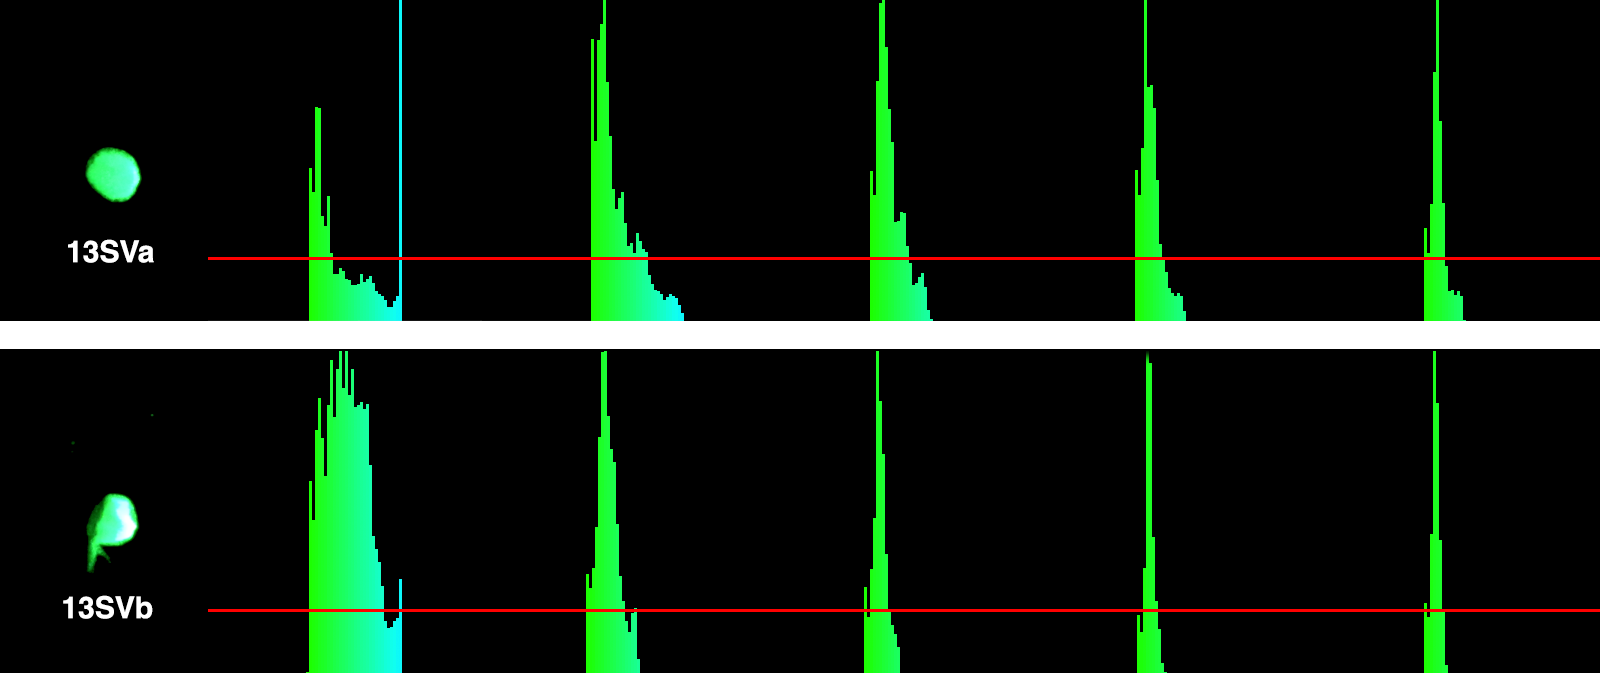
\includegraphics[page=1,width=\textwidth]{images/findings/13SV}
  \caption{Due to an artefact introduced during the taggant preparation the first two samples of taggant \emph{13SVb} were largely dissimiliar compared to its sibling \emph{13SVa}. The red horizontal line depicts the persistance threshold.}
  \label{figure:13SV}
\end{figure}

Based on Figure \ref{figure:tags_presets} increasing $B_{count}$ from three to six fingerprints seems to have minimal effect on the number of matches found. The success rate and precision curves given in Figures \ref{figure:match_precision_fingerprint} and \ref{figure:match_precision_histogram} support this observation: after a certain level of $B_{margin}$ the success rate stagnates regardless of the $B_{count}$, while precision continues to decrease. Moreover, a combination of a high $B_{count}$ and $B_{margin}$ degrades user experience as a larger number of matches (products) would be retrived for the user to choose from. An ideal combination of $B_{margin}$ and $B_{count}$ seems to range from 50-80\% and 3-6 for the fingerprint method, and from 20-40\% and 3-8 for the histogram method. If anything, excessively increasing $B_{margin}$ will only lead to more false positives for the user to filter. On the other hand, as seen in Table \ref{table:match_precision_count1}, if only the best match ($B_{count} = 1$) was processed, the user would be displayed the correct product in less than 50\% of the time, regardless of the method.

As indicated by the clustering in Figure \ref{figure:clusters} and the match distributions in Figure \ref{figure:tags_presets} taggants \emph{24VP} and \emph{24SP} provide good results, especially with presets of the 600ms interval -- higher pigment concentrations seem to improve the SNR. When the boundary conditions are set to $B_{count} = 4$ and $B_{margin} = 30\%$ the success rate and precision of \emph{24SP} is 100\% and 84,26\%, and respectively 94,44\% and 57,35\% for \emph{24VP} using the histogram method. Given this it is surprising that the performance of \emph{24SV} is significantly worse (success rate: 55\%, precision: 46\%). The raw data shows that \emph{24SV} actually comes very close to matching its siblings. In 16 out of the 18 tracings (9 presets $\times$ 2 samples) 50-100\% of the matches included the correct taggant (\emph{24SV}). Thus, the low the success rate of \emph{24SV} was largely due to the given method's inability to distinguish between presets. The $50\mu l$ addition of the green and blue pigments (\emph{G} and \emph{DB}) was not enough to produce any significant change in the emission as illustrated by Figure \ref{figure:SV} -- pigment \emph{DB} attenuates too \emph{slowly} for the samrtphone camera sensor to capture any change. In general however, both of the methods were better at distinguishing the fingerprints by taggant rather than by preset as shown in Table \ref{table:match_precision_count1}.

\begin{figure}[h!]
  \centering 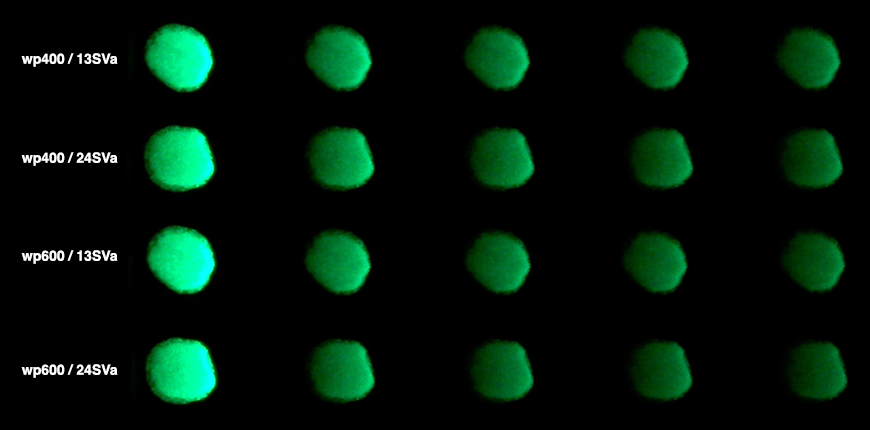
\includegraphics[page=1,width=\textwidth]{images/findings/SV}
  \caption{Regardless of the increase in luminophore concentration and capture interval duration from 400ms to 600ms no significant changes could be observed between taggants \emph{13SV} and \emph{24SV}.}
  \label{figure:SV}
\end{figure}

Overall the histogram method performs better than the fingerprint method. The fingerprint method provides a success rate of approximately 65\% at best, while the success rate of the histogram method ranges up to 95\%. Interestingly enough the maximal success rates are already indicated by Figure \ref{figure:clusters} in how many fingerprints the clusters cover (137 vs. 96 out of 144). Perhaps one equally descriptive metric of the performance of the two methods is the ratio of misses, which is twice as high when using the fingerprint method with $B_{count} = 1$ as shown in Table \ref{table:match_precision_count1}. Based on the standard deviation and mean of $B_{margin}$ visualized in Figure \ref{figure:match_precision_margin} the histogram method is also better at separating (distinguishing) the fingerprints from one antoher as the margin (y-axis) -- within which the matches fit -- is bigger (up until $B_{margin} \approx 85\%$). The tradeoff of the more accurate histogram method is the increase in required computation time and storage space (and bandwidth).

The most significant pitfall of the fingerprint method is the static nature of its analysis parameters. Figure \ref{figure:fingerprint-method-pitfalls} illustrates two example cases where this causes problems. The raw result data revealed that fingerprint \emph{wp\_600/13VPb} matched the rest of the corpus poorly when compared using the fingerprint method. This was due to the excessive number of peaks found in its fourth sample, which in turn resulted in relatively high $P_{hue}$ and $P_{int}$ scores. A fixed persistance threshold -- depicted by the red line in Figure \ref{figure:fingerprint-method-pitfalls} -- worked poorly as the SNR of a sample (frame) decreased (left image). Moreover, using a fixed threshold the fingerprint method was unable to account for slight variations in the hue distribution caused by e.g. residual afterglow from a previous capture as seen in Figure \ref{figure:fingerprint-method-pitfalls} on the right.

While increasing the size of the hue bins based on SNR could address these issues, it would become questionable whether or not the latter fingerprint samples (4th and 5th frame) could provide any useful information. Perhaps a better approach would be to improve the SNR itself e.g using a more novel filtering technique. Outstanding challenges and prospects for future work are discussed further in the next chapter.

\begin{figure}[h!]
  \centering 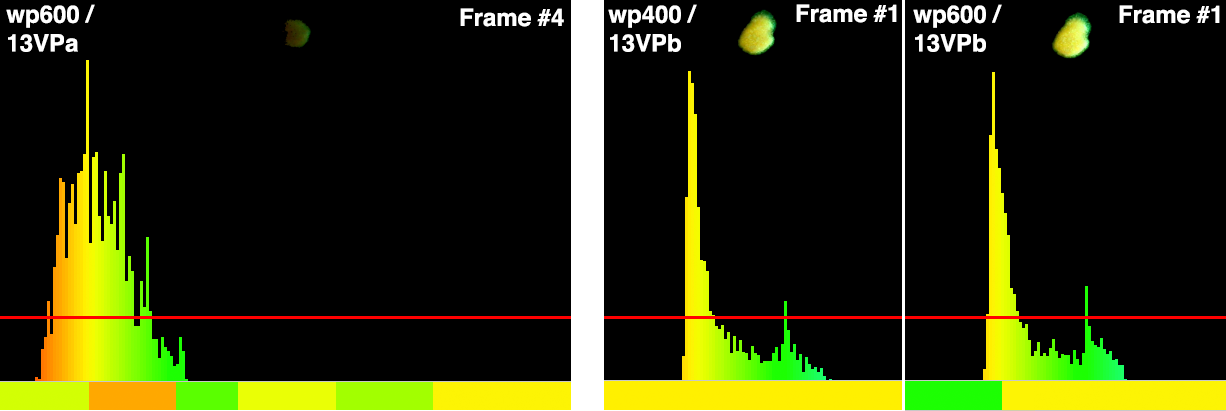
\includegraphics[page=1,width=\textwidth]{images/findings/persistance_pitfall}
  \caption{A fixed persistance threshold (red line) provided inaccurate results when SNR was low (left image). Moreover, a fixed persistance threshold was unable to account for slight variations in the hue distribution -- caused by e.g. residual afterglow from a previous capture -- leading to inconsistent results (right image). The color bars on the x-axis depict the relative amounts of different hues in the histogram.}
  \label{figure:fingerprint-method-pitfalls}
\end{figure}
\clearpage

Based on the results presented in Chapter \ref{chapter:results} and the findings above the following is concluded:

\begin{enumerate}
  \item The histogram method performs better overall, but the fingerprint method allows stricter space and time requirements
    \begin{itemize}
      \item proposed fingerprint method $B_{margin}$ and $B_{count}$: 50-80\% and 3-6
      \item proposed histogram method $B_{margin}$ and $B_{count}$: 20-40\% and 3-8
      \item boundary conditions could be adjusted as per user feedback (e.g. implementing a \emph{Show more} functionality)
    \end{itemize}
  \item Longer intervals provide better results, but have implications for user experience and depend largely on the taggant's excitation lifespan
  \item Lumia 1020 outperforms the Samsung S4 due to its better quality (less noisy) sensor and the artefacts inherent in the Samsung S4
  \item Taggant preparation has a significant impact on the tracing
    \begin{itemize}
      \item sibling taggant shape and size (concentration) should be identical
      \item the luminophore should be fast enough for any significant change to be detected (preferably an excitation lifespan of \textless\ 5000ms)
      \item the absorption wavelength of the luminophore should be close to the wavelength of the light source
    \end{itemize}
  \item The performance of the fingerprint could likely be improved by better noise filtering and adapting the persistance threshold based on SNR.
\end{enumerate}


\section{Challenges and Future Work}

The primary challenge in systems that rely on color information -- be it an image of a taggant or its emission spectrum -- is color calibration. As RGB is a device-dependent color model, different smartphones detect and reproduce a given RGB value differently: the sensor's response to the individual R, G, and B levels vary from vendor to vendor -- or even in the same device over time due to e.g. fabrication and aperture variations. Thus, an RGB value does not define the same color across devices without some kind of color management process.

There are mainly two modules responsible for the color management (color correction) of a digital instrument: illuminant estimation (capture context) and color matrix transformation (color profile), the purpose of which is to transform the sensor output to a standard (rendered) color space. The capture context could be made constant by using the same camera module (and the associated light source), but color profiles would still need to be created separately for each supported smartphone model. Furthermore, the sensor data would need to be captured in RAW format, since a color profile is only really useful when it is applied to \emph{unrendered} sensor data. Thus, color calibration would have implications for both scalability (color profile creation) and performance (RAW image capture). \cite{multiple_cameras} \cite{color_correction_pipeline}

Perhaps a better approach would be to omit color calibration altogether, and instead, have one fingerprint database per each smartphone model. This would offload the complexity of the normalization to the storage layer, where each database would contain the fingerprint corpus captured using a given smartphone model. The impact on scalability would also be minimal as NoSQL databases are typically \emph{horizontally scalable} \cite{nosql_scalability}. To further improve the accuracy of the pipeline additional selection criterion, such as structural and spatial similarity, could be applied. For example, taggants of various shapes and sizes could be used to form a discrete pattern allowing the matching algorithm measure similarity by one more dimension. % Spectra Systems \& CryptoGlyph

Due to the lack of support for burst mode and timed capture by the camera API of both Android 4.4.2 and Windows Phone 8.1 images needed to be captured using the preview frame feed. This was unideal for two reasons. First, the preview feed degrades image quality for better FPS. Second, the application logic required for implementing the capture of the image data from the preview feed incurred additional complexity. Furthermore, in the case of Android, artefacts were introduced. As smartphone camera APIs continue to mature, new capture methods like burst mode will hopefully provide a more stable and higher quality approach to scheduling the capture of multiple frames. In the interim, the use of high definition video remains an intriguing -- although perhaps equally challenging -- alternative.

Regardless of the above mentioned corpus normalization techniques, additional selection semantics or the capture logic, the methods presented in this thesis for analyzing and matching fingerprints remain applicable. As realised in the previous chapter, the histogram method is the preferred method for matching fingerprints. The fingerprint method could still, however, prove useful as a fingerprint \emph{descriptor} for querying and filtering larger sets of fingerprints (e.g. a database). Its apparent pitfalls, as introduced in Chapter \ref{chapter:findings}, would need to be addressed first by implementing a more novel analysis algorithm for filtering and peak finding.

Equally important to that of the capture and analysis methods are the luminous properties of the taggants and the light source. The LumiNova\textregistered\ pigments -- originally developed for use in watch dials -- used in the experiment were not entirely ideal test subjects. Their relatively long excitation lifetime made them difficult to differentiate. Ideally, the full-spectrum white light source used for the photoexcitation would also have been replaced by a less powerful light source of a specific wavelength range for a more controlled and realistic experimentation setting. The light source should be small to be practical but also powerful enough to excite the taggant. A light source emitting a specific wavelength range would likely be better than a general purpose full-spectrum white light. However, as different luminophores have different excitation wavelength ranges, the question becomes which wavelength range the light source should cover?


% The excitation wavelength of a luminophore can be artifically

- idempotence of the luminphores (photobleach)
- cost of artificial fabrication


APP
- change management / how to handle updates \& different devices?
- device detection (automatic configuration, database per phone model), scalability concerns
- easily extendable due to iOS (due to hybrid approach) support (ios with c++? On iOS this extra bridge is unnecessary as C++ code can directly invoke Objective-C APIs.)

CLOUD
- more efficient/safer matching if done server-side (leverage histogram data directly?)
  - easy to switch over because the offline-first approach taken
Attack scenarios
- get hold of the device or man-in-the-middle (metadata works as a layer of indirection)
using a predefined username and password (easily extendable to a real user auth)
- CouchDB uses a traditional cookie based authentication scheme, and as such, applications can be vulnerable to CSRF attacks. However, the application has no CSRF attacks vectors as it the DBMS and the application server is read-only
Traditional Cookie-Based Auth (could be extended to Modern Token-Based Auth such as JWT)


\begin{itemize}
  \item \textbf{RQ1}: How can photoluminescence and smartphones be integrated for product authentication purposes?
  \item \textbf{RQ2}: Which factors affect the analysis of photoluminescent material in the context of smartphones?
  \item \textbf{RQ3}: Does modern smartphone technology provide the means for photoluminescence based product authentication in practice?
    Artificial, customized luminophores
\end{itemize}

\end{document}